%% Indian Journal of History of Science submission (Springer Nature template, author-year references)
\documentclass[pdflatex,sn-basic]{sn-jnl}

\usepackage{graphicx}
\usepackage{amsmath,amssymb,amsthm}
\usepackage{booktabs}
\usepackage{array}
\usepackage{tikz}
\usetikzlibrary{arrows.meta,positioning}
\usepackage{url}

\theoremstyle{thmstyleone}
\newtheorem{theorem}{Theorem}
\newtheorem{lemma}[theorem]{Lemma}
\newtheorem{proposition}[theorem]{Proposition}
\newtheorem{corollary}[theorem]{Corollary}
\theoremstyle{thmstylethree}
\newtheorem{definition}{Definition}
\newtheorem{hypothesis}{Hypothesis}

\newcommand{\Fact}{\textsf{[F]}}
\newcommand{\Schol}{\textsf{[S]}}
\newcommand{\Hyp}{\textsf{[H]}}
\newcommand{\sq}[9]{\begin{smallmatrix}#1&#2&#3\\#4&#5&#6\\#7&#8&#9\end{smallmatrix}}

\raggedbottom
\emergencystretch=2em

\begin{document}

\title[The Kubera Yantra]{The Kubera Yantra: Textual Lineage, Combinatorial Structure, and an Emic Reconstruction of a $3\times3$ Wealth Cosmogram}

\author*[1]{\fnm{Sangaraju Vikram} \sur{Varma}}\email{CORRESPONDING-EMAIL}

\affil*[1]{\orgname{Independent Researcher}, \orgaddress{\city{Bangalore}, \country{India}}. ORCID: 0009-0000-5368-503X}

\abstract{The Kubera Yantra, a $3\times3$ array of the integers 20--28 whose rows, columns and diagonals all sum to 72, is widely drawn and sold in India, but most claims about it are unsourced. This article traces the deity and the ritual attached to the yantra through primary texts, from Atharvaveda 8.10.28 and the Vai\'srava\d na rite of Taittir\=\i ya \=Ara\d nyaka 1.31 to the R\=am\=aya\d na, the Mah\=abh\=arata, the Amarako\'sa, the Kul\=ar\d nava Tantra, the Mantramahodadhi (1588 CE) and the Dharmasindhu. It locates the widely chanted 35-syllable Kubera mantra at Mantramahodadhi 16.105--107 and the Ekapi\.ngala episode at R\=am\=aya\d na 7.13.21--30. It proves, with exhaustive computation, that the Kubera square is the Lo Shu reflected and translated by 19, and the only one of 114 essentially distinct $3\times3$ magic squares with sum 72 built on consecutive integers. Var\=ahamihira's perfume square and the Khajuraho square are re-verified as pandiagonal. Finally, the tradition's own account of how the yantra draws and keeps wealth is reconstructed from its premises, with every claim graded as textual fact, interpretation or hypothesis.}

\keywords{Kubera yantra, magic squares, Lo Shu, history of Indian mathematics, Var\=ahamihira, Mantramahodadhi, Sanskrit ritual texts, yantra, kolam}

\maketitle

\section{Introduction}
The square
\begin{equation}
K=\begin{pmatrix}27&20&25\\22&24&26\\23&28&21\end{pmatrix}
\label{eq:K}
\end{equation}
is sold, painted and drawn across India as the \emph{Kubera Yantra}, a device associated with Kubera (Vai\'srava\d na), guardian of wealth and of the northern quarter. Wikipedia's \emph{Kuberakolam} entry records the same array as a rice-flour floor drawing in South India, gives a drawing order for the numerals, and notes a steganographic use \citep{wiki_kuberakolam}. Beyond that, most claims in circulation lack sources.

The object sits where three literatures meet: the history of magic squares in China, India and the Islamic world \citep{cammann1960,cammann1961,cammann1969a,cammann1969b,hayashi1987,datta1992,swetz2008}; the textual history of Kubera and of yantra worship \citep{sutherland1991,buhnemann2000}; and computational uses of kolam patterns \citep{amirtharajan2013}. No study we know of brings the three together for this particular square, and none separates what the texts actually say from later accretion.

\paragraph*{Epistemic labels} Every substantive claim carries one of three labels: \Fact{} for a statement read directly in a cited primary text or a verified computation; \Schol{} for an interpretation established in peer-reviewed scholarship; \Hyp{} for this paper's own synthesis or proposed reading. Hypotheses are offered for testing and are not presented as findings.

\paragraph*{Contributions}
\begin{enumerate}
\item A source-verified textual dossier on Kubera, his mantras and his ritual (Sec.~\ref{sec:texts}), with corrected references for several widely repeated claims (Table~\ref{tab:corrections}).
\item Theorems, with machine-checked proofs, on the structure of the Kubera square and its family, and a recomputation of the order-4 Indian squares (Sec.~\ref{sec:math}).
\item A cosmogram analysis of the grid under five drawing conventions (Sec.~\ref{sec:cosmo}).
\item A cross-cultural comparison of planetary and wealth squares, and a measured toy experiment on Kubera-ordered steganography (Sec.~\ref{sec:cross}).
\item An emic reconstruction, built only from the tradition's own premises, of how the yantra is held to ``attract and retain'' wealth (Sec.~\ref{sec:emic}).
\end{enumerate}

% =====================================================================
\section{Related Work}
\label{sec:related}
\emph{Magic squares.} Cammann's studies remain the standard account of the Chinese order-3 square (Lo Shu) and of Islamic and Indian squares \citep{cammann1960,cammann1961,cammann1969a,cammann1969b}. Swetz surveys the Lo Shu across cultures \citep{swetz2008}. For India, Datta and Singh's survey (revised by Shukla) \citep{datta1992}, Hayashi's analysis of Var\=ahamihira's pandiagonal square \citep{hayashi1987}, the SaKHYa edition of Thakkura Pher\=u's Ga\d nitas\=arakaumud\=\i{} \citep{sakhya2009}, Singh's work on N\=ar\=aya\d na Pa\d n\d dita's Ga\d nitakaumud\=\i{} (1356) \citep{singh1998}, and Plofker's synthesis \citep{plofker2009} are the main references. None of these, as far as we could determine, discusses the Kubera square specifically.

\emph{Kubera, yak\d sas and Tantric iconography.} Sutherland traces the yak\d sa from Vedic to Buddhist sources \citep{sutherland1991}; Coomaraswamy's \emph{Yak\d sas} is the classic art-historical study \citep{coomaraswamy1928}; Getty records Buddhist Jambhala and Vai\'srava\d na iconography \citep{getty1914}. B\"uhnemann's edition and translation of the Mantramahodadhi's meditation verses \citep{buhnemann2000} is the basis for our reading of that text's Kubera passages. A 2018 article on the Vai\'srava\d na rite of the Taittir\=\i ya \=Ara\d nyaka exists \citep{joi2018vaisravana}; we know it only from its abstract.

\emph{Kolam and computing.} \citet{amirtharajan2013} used the Kubera kolam to order pixel embedding in random image steganography.

% =====================================================================
\section{Sources and Method}
\label{sec:method}
\emph{Corpus.} Sanskrit texts were read in GRETIL e-texts derived from critical or standard editions (R\=am\=aya\d na, Mah\=abh\=arata, Amarako\'sa, M\=arka\d n\d deya, Matsya, B\d rhatsa\d mhit\=a, B\d rhad\=ara\d nyaka) \citep{gretil_ramayana,gretil_mbh12,gretil_amara,gretil_mkp,gretil_matsya,gretil_bs,gretil_bau}; in the TITUS edition (Atharvaveda) \citep{titus_avs}; and in OCR text of printed editions on the Internet Archive (Taittir\=\i ya \=Ara\d nyaka with S\=aya\d na \citep{mitra1872ta}, Kul\=ar\d nava Tantra \citep{kularnava1917}, Dharmasindhu \citep{dharmasindhu1907}, Mantra Mah\=ar\d nava \citep{mantramaharnava}). Translations were used for checking and quotation \citep{roy_santi2,dutt1896mkp,mm1988trans,buhnemann2000,eggeling1900sbe44,agrippa1651}.

\emph{Protocol.} For each claim we (i)~located the passage by string search in the e-text; (ii)~read the surrounding context; (iii)~recorded the edition's own numbering; (iv)~where OCR was the only access, quoted only what was legible and flagged reconstruction. Claims we could not trace to a primary text are listed as unverified (Sec.~\ref{sec:disc}).

\emph{Use of AI tools.} In line with the journal's policy, the author records that large-language-model assistants were used to help locate passages in digitised editions, to draft parts of the text and of the verification code, and to typeset the manuscript. Every cited passage was checked by the author against the edition named, every computation was re-run, and the author takes full responsibility for the content.

\emph{Computation.} Six Python scripts (see Code availability) check every mathematical statement by exhaustive enumeration or exact arithmetic, regenerate the figures, and write a log (\texttt{results.txt}).

% =====================================================================
\section{Textual Lineage}
\label{sec:texts}

\subsection{Vedic layer: concealment, the north, and the Vai\'srava\d na rite}
\emph{Atharvaveda (\'Saunaka) 8.10.28} \Fact. In the Vir\=aj hymn, the cosmic cow goes to each class of beings, who ``milk'' a characteristic power from her. She comes to the \emph{itarajan\=a\d h} (``other folk''), who call her \emph{tirodha} (``Concealment''); her calf is \emph{kubero vai\'srava\d na\d h}, her vessel an unbaked pot, and the milker Rajatan\=abhi K\=aberaka ``milked from her concealment (\emph{tirodh\=a}) alone''; one who knows this ``conceals all evil'' \citep{titus_avs}.

\emph{\'Satapatha Br\=ahma\d na 13.4.3.10} \Fact. In the cycle of Horse-Sacrifice narratives, the day's king is ``King Kubera Vai\'srava\d na''; his people are the Rak\d sas, represented in the assembly by ``evil-doers, robbers'', and a Devajana-vidy\=a is recited \citep{eggeling1900sbe44}.

\emph{Taittir\=\i ya \=Ara\d nyaka 1.31} \Fact. S\=aya\d na introduces this anuv\=aka as the mantras of the \emph{vai\'srava\d na-yaj\~na} and says that Vai\'srava\d na is invoked with four verses \citep{mitra1872ta}. The verses (i)~open with \emph{adbhyas tirodh\=aj\=ayata}, ``Concealment was born from the waters,'' and ask the god to ``conceal'' (\emph{tirodhehi}) the worshipper's rivals; (ii)~summon him on a Tva\d s\d t\d r-made chariot, as one ``to whom beings bring tribute: wealth, cows, elephants, gold, horses''; (iii)~pray to stand in the favour of the one ``who bears \'Sr\=\i{}, the food-faced Vir\=aj'' (\emph{\'sriya\d m bibhrato 'nnamukh\=\i\d m vir\=ajam}); and (iv)~name his city on Mounts Sudar\'sana, Krau\~nca and Main\=aka. The ritual prose (the \emph{kalpa}) gives a bali formula to ``Hira\d nyan\=abhi, Vitudi, the Kaubera'' and an address: ``You, Vai\'srava\d na, are \emph{k\d satra}; we are br\=ahma\d nas \dots{} do not harm me.'' The fire is installed with \emph{tirodh\=a bh\=u\d h sv\=ah\=a} formulas. The rite is done when all oblations have been offered, or after people are asleep. It must not be taught to the careless, and ``for those who do not know it, hungry, no aims succeed.'' In kandik\=a~5 the worshipper offers the first ball to ``your obstructive brother (\emph{vigh\=atuko bhr\=at\=a}) who has settled within my heart'' so that he ``may not destroy my aims'' (\emph{sa me 'rth\=an m\=a vivadh\=\i t}). Kandik\=a~6 then gives the verse \emph{r\=aj\=adhir\=aj\=aya prasahyas\=ahine} (Table~\ref{tab:mantras}). S\=aya\d na glosses \emph{k\=ame\'svara} as ``lord of all desires.'' On the rite's timing he quotes Baudh\=ayana: the vai\'srava\d na-yaj\~na is for one who desires food, or all desires, and is performed ``at every parvan,'' that is, at each new and full moon. We read all of this in the OCR of Mitra's 1872 edition. Prap\=a\d thaka~1, anuv\=aka~31 runs over pp.~181--187, and kandik\=a~6 closes with the marker ``$\|$\,6\,$\|$''.

\emph{Interpretive note} \Schol/\Hyp. The \emph{tirodh\=a}~(concealment) motif links AV~8.10.28 and TA~1.31. The 2018 article cited above argues from its abstract that Vai\'srava\d na may originally have been a spirit of concealment \citep{joi2018vaisravana}. We add a linguistic observation \Hyp: \emph{tiro-dh\=a} (``putting out of sight'') and \emph{ni-dhi} (``deposit, treasure'') are both built on the root \emph{dh\=a}, ``to place.'' On this reading, Kubera's treasure is wealth that has been \emph{put away}. S\=aya\d na also seems to read \emph{prasahyas\=ahin} as one who can forcibly \emph{block} gains, but the OCR of this gloss is damaged. If that reading holds, then together with the ``obstructive brother in my heart'' the Vedic Kubera appears as a \emph{withholder} of wealth who is propitiated so that he will release it.

\subsection{Epic layer}
\emph{R\=am\=aya\d na, critical text} \Fact{} \citep{gretil_ramayana}. Vai\'srava\d na is the son of Vi\'sravas by Bharadv\=aja's daughter (7.3.3--7). After a thousand years of austerity he asks Brahm\=a for ``guardianship of the world, protection of wealth'' (\emph{lokap\=alatvam iccheya\d m vittarak\d sa\d nam}, 7.3.14). Brahm\=a makes him the fourth lokap\=ala after Yama, Indra and Varu\d na (7.3.16--17) and gives him the Pu\d spaka (7.3.18). Vi\'sravas assigns him La\.nk\=a (7.3.24--27). When R\=ava\d na later demands La\.nk\=a, Vi\'sravas advises his son to withdraw to Kail\=asa (7.11.27--41). The \emph{Ekapi\.ngala} story is in 7.13.21--30: while Kubera is performing a vow on the Himalaya, his \emph{left} eye falls on P\=arvat\=\i{} and is scorched by her power, so that it turns yellow (\emph{pi\.ngalatvam}). \'Siva, pleased by Kubera's 800-year vow, offers him friendship (\emph{sakhitva}, 7.13.29) and declares that the name ``Ek\=ak\d si-pi\.ngala'' will last forever (7.13.30). R\=ava\d na takes the Pu\d spaka at 7.15.29.

\emph{Mah\=abh\=arata 12.221, the \'Sr\=\i{}--\'Sakra dialogue} \Fact{} \citep{gretil_mbh12,roy_santi2}. In the critical edition this is \'S\=antiparvan 12.221; in the vulgate followed by Ganguli it is Section CCXXVIII. \'Sr\=\i{} names herself \emph{lak\d sm\=\i}, \emph{bh\=uti} and \emph{\'sr\=\i} (12.221.21). She dwells with victorious kings, with the steadfast, the truthful, the humble and the generous (12.221.23--25). ``Formerly I dwelt among the asuras because they were bound to truth and dharma; finding them reversed, I chose to dwell in you'' (12.221.26). Among the asuras' former virtues she lists well-swept houses (\emph{susa\d mm\d r\d s\d tag\d rh\=a\d h}, 12.221.30), rising before the sun (12.221.36), always giving and never receiving (12.221.38), and never eating fine food alone (12.221.43). Her reasons for leaving include admiring wealth won by adharma (12.221.53), eating without first giving to the gods, ancestors, guests and dependants (12.221.56, 61), grain left scattered for crows and rats and household implements strewn about (12.221.58--59), and sleeping past sunrise (12.221.63). Seven goddesses accompany her, and an eighth leads them (12.221.81--83). The critical text names them \emph{\=a\'s\=a, \'sraddh\=a, dh\d rti, k\=anti, vijiti, sannati, k\d sam\=a} with \emph{v\d rtti} as the eighth; the vulgate rendered by Ganguli has Jay\=a as the eighth.

\subsection{Lexical and Pur\=a\d nic layer}
\emph{Amarako\'sa} \Fact{} \citep{gretil_amara}. The synonym list for Kubera includes \emph{tryambakasakha} (``friend of \'Siva''), \emph{dhanada}, \emph{r\=ajar\=aja}, \emph{vai\'srava\d na}, \emph{narav\=ahana}, \emph{ekapi\.nga}, \emph{ailavila} and \emph{\'sr\=\i da}, ``giver of \'Sr\=\i'' (e-text 1.1.157--160). The nine treasures are \emph{mah\=apadma, padma, \'sa\.nkha, makara, kacchapa, mukunda, kunda, n\=\i la, kharva} (1.1.165--166). The guardians of the quarters, taken from the east, are Indra, Agni, Yama, Nair\d rta, Varu\d na, Marut, \emph{Kubera} (north) and \=I\'sa (1.3.178--179).

\emph{M\=arka\d n\d deya Pur\=a\d na 68} \Fact{} \citep{dutt1896mkp,els_mkp68}. The \emph{Padmin\=\i{} vidy\=a} has Lak\d sm\=\i{} as its presiding deity and the \emph{nidhis} as its supports. It lists \emph{eight} nidhis: padma, mah\=apadma, makara, kacchapa, mukunda, nandaka, n\=\i la and \'sa\.nkha (68.5). Each nidhi has a gu\d na and, by its ``glance,'' shapes the character of the person who holds it. The holder of \'Sa\.nkha, for example, eats fine food himself while his family and servants eat poorly (68.42--45). The chapter ends with the statement that the Padmin\=\i{}, ``of the nature of Lak\d sm\=\i,'' controls them all (68.47). Elsewhere in the same Pur\=a\d na, the Dev\=\i m\=ah\=atmya has \'Sumbha's servants report that the Mah\=apadma treasure was ``brought from Dhane\'svara'' (GRETIL 85.52) \citep{gretil_mkp}.

\emph{Matsya Pur\=a\d na 93.10--12} \Fact{} \citep{gretil_matsya}. In the graha-ma\d n\d dala the Sun sits at the centre, Mars in the south, \emph{Jupiter in the north}, Mercury in the north-east, Venus in the east, the Moon in the south-east, Saturn in the west, R\=ahu in the south-west and Ketu in the north-west.

\subsection{Tantric and ritual layer}
\emph{Yantra theory: Kul\=ar\d nava Tantra 6.85--87} \Fact{} \citep{kularnava1917}. ``The yantra is said to consist of mantra; the deity has mantra as her form; worshipped in the yantra she is pleased at once (85). Because it restrains (\emph{niyantra\d n\=at}) all sorrow born of faults such as desire and anger, it is called \emph{yantra} (86). As the body is to the soul and oil to the lamp, so the yantra is established for all the gods (87).''

\emph{Mantramahodadhi (Mah\=\i dhara, dated by its colophon to 1588 CE \citep{buhnemann2000})} \Fact{} \citep{mm1988trans,buhnemann2000}. Tara\.nga 9.80--84 gives an eight-syllable mantra, \emph{o\d m vai\'srava\d n\=aya sv\=ah\=a}, with a fire-ritual meditation: Kubera in the fire, holding a golden pot full of money and a box of jewels, short-limbed and pot-bellied, under a banyan tree. This Kubera rite closes the section on the worship of Bh\=u and \'Sr\=\i{} \citep{buhnemann2000}. Tara\.nga 16.105--111 gives the \textbf{35-syllable mantra} (Table~\ref{tab:mantras}): seer Vi\'sravas, metre B\d rhat\=\i, deity ``lord of wealth, friend of \'Siva.'' The six-limbed placement (\emph{\d sa\d da\.nga-ny\=asa}) divides it into $3,4,5,8,8,7$ syllables. The meditation verse (16.109) begins \emph{manujav\=ahyavim\=anavarasthita\d m} (``seated in a fine aerial car borne by men''). The procedure is $10^5$ repetitions with $10^4$ sesame oblations; worship on a seat with Dharma and the other seat-deities, the six limbs, and the quarter-guardians with their weapons; $10^4$ repetitions in a \'Siva temple ``for increase of wealth''; and $10^5$ repetitions seated at the root of a bilva tree. Tara\.nga 16.112--113 adds a 16-syllable mantra addressed to \emph{Vitte\'svara}. Tara\.nga 20.1--14 gives the general procedure for yantras. If no material is specified, the yantra is written on birch-bark (\emph{bh\=urja}), silk or palm leaf; it is worshipped with japa and homa, soaked in the residue of the oblation ghee, sealed in a gold, silver or copper amulet, and the life-installation (\emph{pr\=a\d napratis\d th\=a}) mantra is written around it.

\emph{Mantra Mah\=ar\d nava} \Fact{} \citep{mantramaharnava}. This later digest reproduces the same 35-syllable mantra, says explicitly that it is taken ``from the Mantra Mahodadhi,'' and specifies the \emph{Kubera p\=ujana yantra}: the image or yantra, made of gold or other metal, is placed in a copper dish, anointed with ghee, bathed with streams of milk and water, set at the centre of a \emph{sarvatobhadra} ma\d n\d dala, and given life-installation. Worship then proceeds through a hexagon (the six limbs) and an outer square (the ten guardians of the quarters).

\emph{Dharmasindhu} \Fact{} \citep{dharmasindhu1907}. On the new-moon night of \=A\'svina, the text prescribes an oil bath in the morning, and at dusk the offering of lamps, the showing of torches and the worship of Lak\d sm\=\i{}. After midnight the women of the town drive \emph{Alak\d sm\=\i} out of their courtyards. A separate \emph{dh\=anya-mantra}, \emph{o\d m dhanad\=aya sarvalokahit\=aya dehi me dh\=anya\d m sv\=ah\=a} (our reconstruction from OCR), is to be written and placed in the granary ``for increase of grain.'' The same passage says that spending wealth or grain on Wednesday or Saturday is not auspicious.

\emph{Buddhist and Jain parallels} \Schol. Vai\'srava\d na is guardian of the north among the Four Great Kings. In Tibetan Buddhism the wealth god Jambhala, with his jewel-spitting mongoose, absorbs Vai\'srava\d na iconography \citep{getty1914,sutherland1991}. Jain iconographic manuals name a yak\d sa Kubera (we did not examine the primary Jain sources).

\subsection{What the texts do \emph{not} contain}
We searched the full OCR of the Mantramahodadhi translation, both Mantra Mah\=ar\d nava scans, the \'S\=arad\=atilaka with R\=aghavabha\d t\d ta's commentary, and the Dharmasindhu for the numerals of $K$, for the word ``72,'' and for numeric Kubera yantras. We found none. The textual \emph{Kubera p\=ujana yantra} is a geometric enclosure diagram (hexagon in a square, with guardians of the quarters), not a magic square. We could not date the first attestation of the numeric square; the earliest dated source we found is Wikipedia's 2013 citation of a devotional web article \citep{wiki_kuberakolam}.

\begin{table*}[t]
\caption{Kubera mantras: text, verified source, and syllable count (counts computed by \texttt{mantra\_syllables.py}).}
\label{tab:mantras}
\centering\small
\begin{tabular}{@{}>{\raggedright\arraybackslash}p{0.36\textwidth}>{\raggedright\arraybackslash}p{0.34\textwidth}>{\raggedright\arraybackslash}p{0.24\textwidth}@{}}
\toprule
Text (IAST) & Word-by-word sense & Source / status \\
\midrule
\emph{r\=aj\=adhir\=aj\=aya prasahyas\=ahine / namo vaya\d m vai\'srava\d n\=aya kurmahe / sa me k\=am\=an k\=amak\=am\=aya mahyam / k\=ame\'svaro vai\'srava\d no dad\=atu / kuber\=aya vai\'srava\d n\=aya / mah\=ar\=aj\=aya nama\d h}
& to the king over kings, to the forceful overpowerer / we make obeisance to Vai\'srava\d na (son of Vi\'sravas) / may he [give] desires to me, desirous of desires / may Vai\'srava\d na, lord of desires, give / to Kubera Vai\'srava\d na / to the great king, homage
& Taittir\=\i ya \=Ara\d nyaka 1.31.6 (Mitra ed.\ 1872) \Fact; p\=adas of 12, 12, 11, 11 syllables; recited in the Mantrapu\d spa after TA 1.22 (liturgical practice) \\
\midrule
\emph{yak\d s\=aya kuber\=aya vai\'srava\d n\=aya dhanadh\=any\=adhipataye dhanadh\=anyasam\d rddhi\d m me dehi d\=apaya sv\=ah\=a}
& to the Yak\d sa, to Kubera, to Vai\'srava\d na, to the overlord of wealth and grain: abundance of wealth and grain to me give, cause to be given (causative \emph{d\=apaya}); sv\=ah\=a
& Mantramahodadhi 16.105--107 \Fact; seer Vi\'sravas, metre B\d rhat\=\i; 35 syllables without \emph{o\d m} (36 with it); \d sa\d da\.nga split 3-4-5-8-8-7 verified \\
\midrule
\emph{o\d m vai\'srava\d n\=aya sv\=ah\=a} & om, to Vai\'srava\d na, sv\=ah\=a & MM 9.81--84 \Fact; 8 syllables \\
\emph{o\d m \'sr\=\i\d m o\d m hr\=\i\d m \'sr\=\i\d m hr\=\i\d m kl\=\i\d m \'sr\=\i\d m kl\=\i\d m vitte\'svar\=aya nama\d h} & seed-syllables; homage to the lord of riches & MM 16.112--113 \Fact; 16 syllables \\
\emph{o\d m dhanad\=aya sarvalokahit\=aya dehi me dh\=anya\d m sv\=ah\=a} & to the wealth-giver, benefactor of all worlds: give me grain & Dharmasindhu III (p\=urv\=ardha) \Fact{} (OCR reconstruction) \\
``Kubera G\=ayatr\=\i'' (\emph{yak\d sar\=aj\=aya vidmahe \dots}) & --- & no classical source found; modern devotional \\
\bottomrule
\end{tabular}
\end{table*}

% =====================================================================
\section{Mathematics}
\label{sec:math}

\begin{definition}
A $3\times3$ array $A=(a_{ij})$ of numbers is \emph{magic} with sum $S$ if all three rows, all three columns and both main diagonals sum to $S$. It is \emph{normal} if its entries are $1,\dots,9$. The group $D_4$ of the eight rotations and reflections of the square acts on arrays; two arrays are \emph{essentially the same} if they lie in one $D_4$-orbit. Write $L$ for the Lo Shu as conventionally printed with south at the top, $L=\left(\sq{4}{9}{2}{3}{5}{7}{8}{1}{6}\right)$ \citep{cammann1961,wiki_luoshu}.
\end{definition}

\begin{lemma}[Centre lemma]\label{lem:centre}
In every $3\times3$ magic array over a field of characteristic $\neq3$, the centre equals $S/3$.
\end{lemma}
\begin{proof}
The middle row, the middle column and the two diagonals together count the centre $c$ four times and every other cell once. So $4S=(\text{sum of all cells})+3c=3S+3c$, and hence $c=S/3$.
\end{proof}

\begin{proposition}[Three-parameter form]\label{prop:lucas}
The magic arrays form a 3-dimensional space. Every one can be written as
\[\begin{pmatrix}c-b&c+a+b&c-a\\c-a+b&c&c+a-b\\c+a&c-a-b&c+b\end{pmatrix}.\]
\end{proposition}
\begin{proof}
The seven equations ``line $=$ first row'' have rank $6$ over $\mathbb{Q}$ (computed exactly). The displayed array is magic for all $a,b,c$, and its three free parameters are the centre, the bottom-left corner minus the centre, and the bottom-right corner minus the centre. Any magic array is therefore determined by those three cells.
\end{proof}

\begin{theorem}[Uniqueness of the normal square]\label{thm:unique}
There are exactly eight normal $3\times3$ magic squares, and they form a single $D_4$-orbit (the orbit of $L$).
\end{theorem}
\begin{proof}
$S=45/3=15$, and by Lemma~\ref{lem:centre} $c=5$. The value $9$ cannot sit in a corner: a corner lies on three lines, and with $9$ in it those three lines need three disjoint pairs from $\{1,\dots,8\}\setminus\{5\}$ summing to $6$, but only $\{1,5\}$ and $\{2,4\}$ do so, and $\{1,5\}$ uses the centre. So $9$ sits on an edge, and $1$ sits opposite it through the centre. The line through $9$ is completed by $\{2,4\}$, the only pair summing to $6$ not using $5$, which fixes two corners. The remaining cells are then forced. There are four edge positions for $9$ and two orders of $\{2,4\}$, giving $8$ squares, all in the orbit of $L$. Exhaustive search over all $9!$ permutations confirms the count (\texttt{magic3.py}).
\end{proof}

\begin{theorem}[Consecutive integers]\label{thm:consec}
Let $A$ be magic with entries $k,k+1,\dots,k+8$. Then $S=3k+12$, the centre is $k+4$, and $A-(k-1)J$ is normal, where $J$ is the all-ones array. There are therefore exactly eight such squares, namely $g(L)+(k-1)J$ for $g\in D_4$.
\end{theorem}
\begin{proof}
The sum of all cells is $9k+36=3S$. The centre follows from Lemma~\ref{lem:centre}. Subtracting a constant from every cell preserves the magic property and maps $\{k,\dots,k+8\}$ onto $\{1,\dots,9\}$. Theorem~\ref{thm:unique} then gives the count.
\end{proof}

\begin{corollary}[Identity of the Kubera square]\label{cor:K}
$K=\rho(L)+19J$, where $\rho$ is the reflection exchanging top and bottom rows. Equivalently, $K-19=\left(\sq{8}{1}{6}{3}{5}{7}{4}{9}{2}\right)$. Its Lucas parameters are $(a,b,c)=(-1,-3,24)$.
\end{corollary}

\begin{figure}[t]
\centering
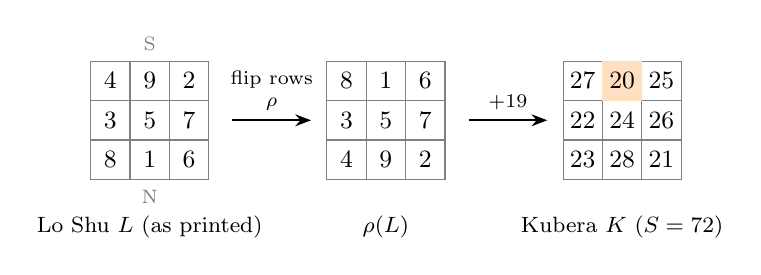
\begin{tikzpicture}[x=0.5cm,y=0.5cm,font=\small]
% Lo Shu (south at top)
\foreach \i/\j/\v in {0/0/4,1/0/9,2/0/2,0/1/3,1/1/5,2/1/7,0/2/8,1/2/1,2/2/6}{
  \draw[gray] (\i,-\j) rectangle ++(1,-1);
  \node at (\i+0.5,-\j-0.5) {\v};}
\node[font=\scriptsize,gray] at (1.5,0.45) {S};
\node[font=\scriptsize,gray] at (1.5,-3.45) {N};
\node[font=\footnotesize] at (1.5,-4.2) {Lo Shu $L$ (as printed)};
% arrow
\draw[-{Stealth[length=2mm]},thick] (3.6,-1.5) -- node[above,font=\scriptsize,align=center]{flip rows\\$\rho$} (5.6,-1.5);
% K-19
\foreach \i/\j/\v in {0/0/8,1/0/1,2/0/6,0/1/3,1/1/5,2/1/7,0/2/4,1/2/9,2/2/2}{
  \draw[gray] (6+\i,-\j) rectangle ++(1,-1);
  \node at (6.5+\i,-\j-0.5) {\v};}
\node[font=\footnotesize] at (7.5,-4.2) {$\rho(L)$};
\draw[-{Stealth[length=2mm]},thick] (9.6,-1.5) -- node[above,font=\scriptsize]{$+19$} (11.6,-1.5);
% K
\foreach \i/\j/\v in {0/0/27,1/0/20,2/0/25,0/1/22,1/1/24,2/1/26,0/2/23,1/2/28,2/2/21}{
  \draw[gray] (12+\i,-\j) rectangle ++(1,-1);
  \node at (12.5+\i,-\j-0.5) {\v};}
\fill[orange!25] (13,0) rectangle (14,-1); \node at (13.5,-0.5) {20};
\node[font=\footnotesize] at (13.5,-4.2) {Kubera $K$ ($S=72$)};
\end{tikzpicture}
\caption{The Kubera square is the conventionally printed Lo Shu with its rows reversed and $19$ added to every cell (Corollary~\ref{cor:K}). The shaded cell, $20$, is the image of the Lo Shu's $1$, the number the Chinese scheme assigns to north.}
\label{fig:LtoK}
\end{figure}
\noindent Among the eight elements of $D_4$, only $\rho$ maps $L$ to $K-19$ (\texttt{magic3.py}, T4). Mirroring $K-19$ left-to-right gives $\left(\sq{6}{1}{8}{7}{5}{3}{2}{9}{4}\right)$, the Lo Shu drawn with north at top and east at right.

\begin{proposition}[How special is 72?]\label{prop:count72}
Up to $D_4$ there are exactly $114$ magic $3\times3$ squares with distinct positive integer entries and $S=72$. Exactly one of them uses nine consecutive integers, and it is $K$.
\end{proposition}
\begin{proof}
By Lemma~\ref{lem:centre}, $c=24$. Proposition~\ref{prop:lucas} reduces the problem to the finitely many $(a,b)$ with $|a|,|b|\le23$. We enumerated them exactly, imposed positivity and distinctness, and reduced modulo $D_4$ (\texttt{magic3.py}, T7).
\end{proof}

\begin{proposition}[Quadratic identities]\label{prop:quad}
In every $3\times3$ magic array, the first and third rows have equal sums of squares, and so do the first and third columns. For $K$ the common values are $1754$ (rows) and $1742$ (columns). Reading the rows of $K$ as base-100 numerals, $272025^2+222426^2+232821^2$ equals the corresponding sum for the reversed rows.
\end{proposition}
\noindent These identities follow from Proposition~\ref{prop:lucas}. They hold for every $3\times3$ magic square, so they say nothing particular about Kubera \Fact.

\begin{table}[t]
\caption{The affine family $L+mJ$: Navagraha sums as commonly published, and Kubera.}
\label{tab:family}
\centering\small
\begin{tabular}{@{}lrrr@{}}
\toprule
Square & offset $m$ & entries & $S=15+3m$\\
\midrule
Sun (S\=urya) & 0 & 1--9 & 15\\
Moon, Mars, Mercury & 1, 2, 3 & \dots & 18, 21, 24\\
Jupiter, Venus, Saturn & 4, 5, 6 & \dots & 27, 30, 33\\
R\=ahu, Ketu & 7, 8 & \dots & 36, 39\\
\textbf{Kubera} & \textbf{19} & \textbf{20--28} & \textbf{72}\\
\bottomrule
\end{tabular}
\end{table}

\begin{figure}[t]
\centering
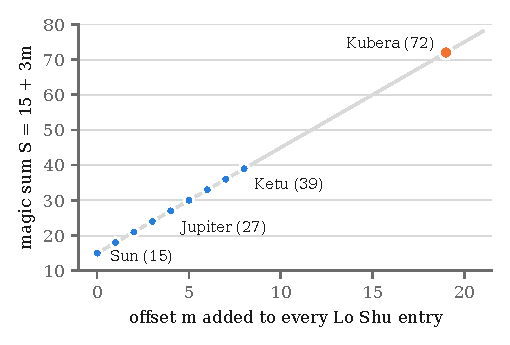
\includegraphics[width=\columnwidth]{figs/fig_family.pdf}
\caption{All $3\times3$ squares on consecutive integers lie on the line $S=15+3m$. The nine Navagraha squares (blue) occupy $m=0,\dots,8$; Kubera (orange) sits at $m=19$, outside that run.}
\label{fig:family}
\end{figure}

\emph{The Navagraha family} \Schol/\Fact. Secondary literature attributes nine planetary $3\times3$ squares to an early author ``Garga'' and reports sums from 15 (Sun) upward in steps of 3 \citep{datta1992,cammann1969b}. We could not examine a primary text for these squares, so Table~\ref{tab:family} gives only the arithmetic. Under Theorem~\ref{thm:consec}, all of these squares are translates of the Lo Shu. The Sun's square is the Lo Shu itself, and Kubera's offset of 19 is not part of that run (Fig.~\ref{fig:family}).

\subsection{Order four: Var\=ahamihira and Khajuraho}
\emph{B\d rhatsa\d mhit\=a 76} \Fact{} \citep{gretil_bs}. Verses 76.23--24 assign proportions to sixteen perfume ingredients in a sixteen-cell \emph{kacchapu\d ta}: $\left(\begin{smallmatrix}2&3&5&8\\5&8&2&3\\4&1&7&6\\7&6&4&1\end{smallmatrix}\right)$. Verse 76.25 states that the four-ingredient combinations amounting to ``eighteen parts'' (\emph{a\d s\d t\=ada\'sa bh\=ag\=a\d h}) are perfumes. Our enumeration confirms that every row, column, main diagonal and broken diagonal, and every wrapped $2\times2$ block, sums to 18. This is consistent with Hayashi's identification of the square as pandiagonal \citep{hayashi1987}. The same chapter also states counts that we checked exactly. Verse 76.20 gives $\binom{16}{4}=1820$ selections, and 76.17 gives $1820\times96=174{,}720$ perfumes. Verse 76.29--30 uses a \emph{nine}-cell kacchapu\d ta from which three substances are drawn, and states that there are 84 \emph{kesara} perfumes, which equals $\binom{9}{3}$. That passage contains no magic numbering. Two normal pandiagonal squares reduce to Var\=ahamihira's square when entries above 8 are reduced by 8 (\texttt{magic4.py}, C4).

\emph{Khajuraho} \Fact. The square on the P\=ar\'svan\=atha temple \citep{oeis_a126710} is pandiagonal and most-perfect. The temple is usually dated to c.\ 950--970; some authors date the inscription of the square later (12th--13th c.) \citep{ahmed2004,oeis_a126710}.

\begin{proposition}[Order-four census]\label{prop:census}
There are $7040$ normal $4\times4$ magic squares ($880$ up to $D_4$). Of these, $384$ are pandiagonal ($48$ up to $D_4$), and every one of the $384$ is most-perfect.
\end{proposition}
\noindent Proof: exhaustive constraint search with forward checking (\texttt{magic4.py}, runtime about 85~s). The 880 agrees with Fr\'enicle's classical count \citep{andrews1917}.

\begin{figure}[t]
\centering
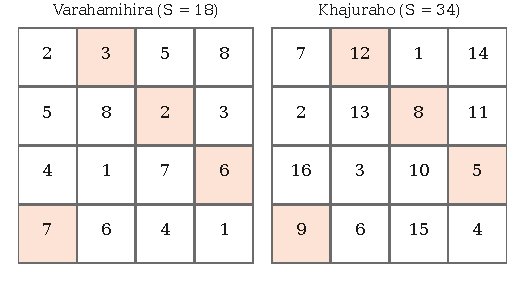
\includegraphics[width=0.92\columnwidth]{figs/fig_squares4.pdf}
\caption{Var\=ahamihira's square (B\d rhatsa\d mhit\=a 76.23--24, sum 18) and the Khajuraho square (sum 34). One broken diagonal is shaded in each; all eight broken diagonals sum to $S$.}
\label{fig:sq4}
\end{figure}

% =====================================================================
\section{The Grid as Cosmogram}
\label{sec:cosmo}
A $3\times3$ grid can be read as the eight quarters around a centre. This is the structure of the guardians of the quarters (Amarako\'sa 1.3), of the graha-ma\d n\d dala (Matsya 93), and, in China, of the Lo Shu read through the Later-Heaven trigram order (1 north, 9 south, 3 east, 7 west, and so on) \citep{cammann1961}. We found no text that fixes which edge of the \emph{numeric} Kubera yantra faces which quarter. We therefore tabulate all conventions (Table~\ref{tab:orient}, Fig.~\ref{fig:orient}).

\begin{table}[t]
\caption{Number of $K$ falling in each quarter, by drawing convention (from \texttt{directions.py}). N = north (Kubera), E = east (Indra), S = south (Yama), C = centre; LH = cells agreeing with the Later-Heaven Lo Shu numbering.}
\label{tab:orient}
\centering\small
\setlength{\tabcolsep}{3pt}
\begin{tabular}{@{}lccccc@{}}
\toprule
Convention & N & E & S & C & LH\\
\midrule
N up, E right (map) & \textbf{20} & 26 & 28 & 24 & 3/9\\
E up, N left (V\=astu) & 22 & 20 & 26 & 24 & 3/9\\
S up, E left (Chinese) & 28 & 22 & 20 & 24 & 3/9\\
N up, E left (mirror) & \textbf{20} & 22 & 28 & 24 & \textbf{9/9}\\
\bottomrule
\end{tabular}
\end{table}

\begin{figure*}[t]
\centering
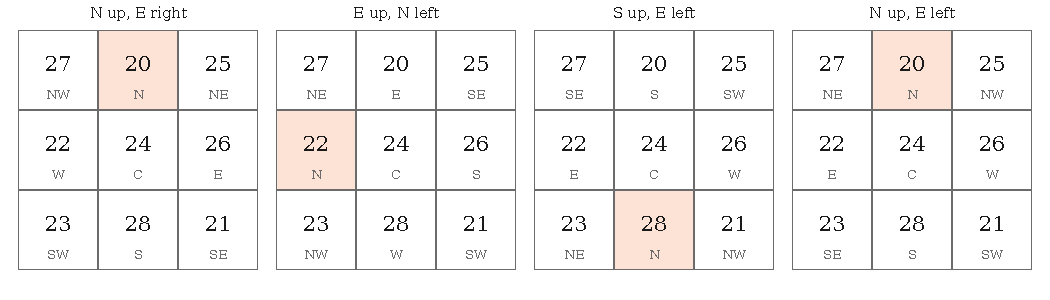
\includegraphics[width=0.85\textwidth]{figs/fig_orient.pdf}
\caption{The Kubera square under four drawing conventions; the cell falling in Kubera's own quarter (north) is shaded. With the top row toward north, the north cell holds 20, which corresponds to the Lo Shu's 1, the number the Chinese scheme assigns to north.}
\label{fig:orient}
\end{figure*}

(1)~\Fact{} The centre is invariant: it always holds 24, which is $S/3$ by Lemma~\ref{lem:centre}. (2)~\Fact{} If the top edge faces north, as with a floor drawing whose top row is laid toward the north, the north cell holds $20$ (Lo Shu $1$) and the south cell $28$ (Lo Shu $9$). The north--south axis then agrees with the Chinese directional numbering and east--west is mirrored. Full agreement (9/9) is obtained only in the mirror convention (north up, east left). (3)~\Hyp{} We therefore read $K$ as a Lo Shu whose \emph{north--south axis} has been kept in cosmographic register, with the smallest number in Kubera's own quarter. Whether anyone designed it so cannot be decided without a dated early exemplar that marks its orientation.

\emph{Negative result} \Fact. If the grahas are numbered in their canonical list order (Sun $=1,\dots,$ Ketu $=9$) and placed as Matsya 93 prescribes, the resulting array is not magic (row sums $18,14,13$). The graha-ma\d n\d dala and the numeric planetary squares are independent systems.

% =====================================================================
\section{Cross-Cultural Comparison and Computing}
\label{sec:cross}
\subsection{Which planet, which square, which wealth?}
In Agrippa's \emph{De occulta philosophia} (1533; English 1651), Book~II, ch.~XXII, the order-3 table belongs to \emph{Saturn} (``in every line three every way, and through each Diameter making fifteen''). Jupiter takes order 4 (sum 34), Mars order 5 (65), the Sun order 6 (111), Venus order 7 (175) and the Moon order 9 (369) \citep{agrippa1651} \Fact. In the Indian Navagraha set as reported in the secondary literature, the order-3 sum-15 square belongs to the \emph{Sun} \citep{datta1992} \Schol. Agrippa connects \emph{riches} not with the 3-square but with Jupiter's 4-square: engraved on a silver plate, it ``conduceth to gain, and riches'' \citep{agrippa1651} \Fact. Both traditions thus attach wealth to a particular magic square on a particular metal \Hyp: India to a translate of the 3-square (Kubera), Renaissance Europe to a 4-square (Jupiter). Matsya 93 places Jupiter in the north, Kubera's quarter. The shared position is suggestive, but it is no evidence of transmission. Islamic \emph{wafq} squares are the documented route that carried magic squares between the Indian and European spheres \citep{cammann1969a,cammann1969b}. We did not investigate the specific question of whether wealth-related uses travelled with them.

\begin{table}[t]
\caption{Order-3 square and wealth square in three traditions.}
\label{tab:cross}
\centering\small
\setlength{\tabcolsep}{3pt}
\begin{tabular}{@{}>{\raggedright\arraybackslash}p{0.20\columnwidth}>{\raggedright\arraybackslash}p{0.36\columnwidth}>{\raggedright\arraybackslash}p{0.36\columnwidth}@{}}
\toprule
Tradition & 3-square assigned to & ``Wealth'' square\\
\midrule
China (Lo Shu) & cosmic diagram, nine halls \citep{cammann1961} & ---\\
India & Sun (Navagraha, secondary sources) & Kubera, $L+19$ (modern devotional)\\
Agrippa (1533) & Saturn \citep{agrippa1651} & Jupiter $4\times4$, silver \citep{agrippa1651}\\
\bottomrule
\end{tabular}
\end{table}

\subsection{Kubera kolam in steganography}
\citet{amirtharajan2013} divide an RGB cover into $6\times6$ blocks. They extend the Kubera square (and its Lo Shu reduction) to fix the visiting order of pixels, and use a pulli-kolam matrix to fix how many bits each pixel carries. To isolate the Kubera contribution we embedded 4480 bits into a synthetic $96\times96$ image, visiting each $3\times3$ block in increasing order of $K$ (\texttt{stego\_demo.py}). The result was PSNR $=54.27$~dB, MSE $=0.243$, and zero bit errors on extraction. Extracting with any of the seven other $D_4$ variants as the ``key'' gave bit-error rates of $0.34$--$0.51$ (Fig.~\ref{fig:stego}). A permutation drawn from ``a magic square of order 3'' carries only $\log_2 8=3$ bits of key. Its contribution to security is therefore small; the interest of the scheme lies in pixel diffusion and in its cultural source \Fact.

\begin{figure}[t]
\centering
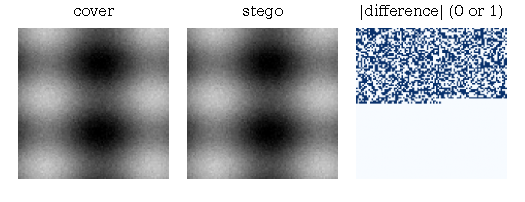
\includegraphics[width=\columnwidth]{figs/fig_stego.pdf}
\caption{Toy Kubera-ordered LSB embedding (synthetic cover, 0.49 bit/pixel over the payload region).}
\label{fig:stego}
\end{figure}

% =====================================================================
\section{An Emic Reconstruction of the Yantra's Logic}
\label{sec:emic}
This section reconstructs, from inside the tradition (\emph{emic}), why a devotee is told the yantra ``attracts and retains'' wealth; no claim about efficacy is made. Each step is labelled; Table~\ref{tab:chain} summarises.

\begin{enumerate}
\item[E1] \emph{Wealth is personified and mobile.} \'Sr\=\i/Lak\d sm\=\i{} chooses where to live and leaves when conduct inverts (MBh 12.221.23--26) \Fact.
\item[E2] \emph{Treasures are under Lak\d sm\=\i's governance.} The nidhis support the Padmin\=\i{} vidy\=a, whose deity is Lak\d sm\=\i{} (MkP 68.4, 47) \Fact.
\item[E3] \emph{Kubera's office is to guard.} He asked for and received \emph{vittarak\d sa\d na}, the protection of wealth (R\=am 7.3.14); he is lord of the nidhis and ``giver of \'Sr\=\i'' (Amarako\'sa) \Fact. In the Vedic rite he is also the one who can withhold, and is propitiated so that he releases (TA 1.31.5--6) \Fact/\Hyp.
\item[E4] \emph{Kubera has a quarter.} North (Amarako\'sa 1.3; R\=am 7.3.16--17) \Fact.
\item[E5] \emph{A yantra is a deity's body.} It consists of mantra, and the deity worshipped in it is ``pleased at once'' (Kul\=ar\d nava 6.85--87). It is enlivened by \emph{pr\=a\d napratis\d th\=a} (MM 20.9--14; Mantra Mah\=ar\d nava) \Fact.
\item[E6] \emph{Effect is conditional on discipline.} Prescribed counts of japa and homa, the place (\'Siva temple, bilva root), and the time (parvan days; the \=A\'svina new moon for Lak\d sm\=\i) are all specified (MM 16.110--111; Baudh\=ayana via S\=aya\d na; Dharmasindhu) \Fact.
\item[E7] \emph{Retention depends on conduct.} Clean house, early rising, sharing food, not admiring ill-gotten wealth, tidy grain stores (MBh 12.221.30--63). MkP 68 attaches the same vice, eating well while dependants go short, to the holder of the \'Sa\.nkha nidhi \Fact. That the two passages express \emph{one} theory of retention is our synthesis \Hyp.
\item[E8] \emph{The grid as balanced cosmos.} The eight lines of $K$ all sum to 72, and every quarter-line through the centre is equal. To the tradition this can figure the balance (\emph{\d rta}, dharma) on which E1 and E7 make \'Sr\=\i{} depend \Hyp. Mathematically, the balance is forced by the arithmetic: Theorem~\ref{thm:consec} shows it holds for any translate of the Lo Shu.
\end{enumerate}

\begin{hypothesis}[Nine cells, nine treasures]\label{hyp:nidhi}
Amarako\'sa lists nine nidhis, and the yantra has nine cells. Writing the list in order onto $20,\dots,28$ puts the fifth nidhi, \emph{kacchapa} (``tortoise''), at the centre (24). In the Chinese legend the Lo Shu itself appeared on a tortoise's back \citep{wiki_luoshu}. Separately, M\=arka\d n\d deya 68 gives \emph{eight} nidhis governed by Lak\d sm\=\i{}, an eight-around-one structure like the eight quarters around a centre.
\end{hypothesis}
\noindent \emph{Status.} No text we examined assigns nidhis to cells. The tortoise coincidence depends on one particular list order, and the list orders of Amarako\'sa and M\=arka\d n\d deya differ. Hypothesis~\ref{hyp:nidhi} is therefore offered only as a mnemonic and devotional reading.

\begin{table}[t]
\caption{Emic chain: claim, evidence, and status.}
\label{tab:chain}
\centering\footnotesize
\setlength{\tabcolsep}{2pt}
\begin{tabular}{@{}p{0.06\columnwidth}p{0.43\columnwidth}p{0.36\columnwidth}p{0.08\columnwidth}@{}}
\toprule
Step & Claim & Evidence & Label\\
\midrule
E1 & \'Sr\=\i{} is mobile, conditional & MBh 12.221.23--26 & F\\
E2 & Lak\d sm\=\i{} governs nidhis & MkP 68 & F\\
E3 & Kubera guards; can withhold & R\=am 7.3.14; TA 1.31.5--6 & F/H\\
E4 & Kubera's quarter is north & Amarako\'sa 1.3 & F\\
E5 & yantra $=$ deity's body & Kul\=ar\d nava 6.85--87 & F\\
E6 & counts, places, times & MM 16.110--111; Dharmasindhu & F\\
E7 & conduct retains \'Sr\=\i & MBh 12.221; MkP 68 & F$+$H\\
E8 & equal sums $\leftrightarrow$ \d rta & Thm.~\ref{thm:consec} & H\\
\bottomrule
\end{tabular}
\end{table}

% =====================================================================
\section{Discussion and Limitations}
\label{sec:disc}
\emph{On 72.} Table~\ref{tab:72} classifies the numerical associations commonly attached to 72. None is attested in connection with Kubera.

\begin{table}[t]
\caption{Associations of 72: status.}
\label{tab:72}
\centering\footnotesize
\setlength{\tabcolsep}{2pt}
\begin{tabular}{@{}p{0.44\columnwidth}p{0.50\columnwidth}@{}}
\toprule
Association & Status\\
\midrule
$72=15+3\cdot19$ (Lo Shu $+19$) & structural (Thm.~\ref{thm:consec}); rationale for 19 unknown\\
72{,}000 \emph{hit\=a} channels (B\d rhad\=ara\d nyaka 2.1.19) \citep{gretil_bau} & attested number; no link to Kubera: coincidence\\
72 mela\-kartas ($2\cdot6\cdot6$) & combinatorial, early-modern music theory: coincidence\\
precession $\approx71.6$ yr/degree & not 72; modern astronomy: coincidence\\
total of cells $216=2\cdot108$ & arithmetic: coincidence\\
\bottomrule
\end{tabular}
\end{table}

\emph{Limitations.} (i)~TA 1.31, Kul\=ar\d nava, Dharmasindhu and Mantra Mah\=ar\d nava were read through OCR of printed editions, and some glosses are damaged. (ii)~We did not access Datta and Singh's full text \citep{datta1992} or a primary source for the Navagraha squares. (iii)~The \'Satapatha passage was located through Eggeling's index rather than a page image. (iv)~The orientation analysis assumes the top edge of the printed yantra is meaningful, which no source states. (v)~Living practice (e.g., Kubera worship on Dhanteras with Lak\d sm\=\i{} on D\=\i p\=aval\=\i{} \citep{drik_kubera_puja}) is documented here only from modern manuals.

\emph{Scope.} The mathematics explains why the square is balanced. Whether the yantra is efficacious is a religious question and lies outside this study.

\begin{table}[t]
\caption{Corrections to frequently repeated claims.}
\label{tab:corrections}
\centering\footnotesize
\setlength{\tabcolsep}{2pt}
\begin{tabular}{@{}p{0.42\columnwidth}p{0.52\columnwidth}@{}}
\toprule
Claim in circulation & Finding\\
\midrule
35-syllable mantra: source unknown & Mantramahodadhi 16.105--107 (1588 CE); 35 excludes \emph{o\d m}\\
Ekapi\.ngala: Pur\=a\d nic & R\=am\=aya\d na 7.13.21--30 (left eye; \'Siva's friendship)\\
``Islamic and Indian Magic Squares'' by Hayashi (Isis) & by Cammann, \emph{History of Religions} 8 (1969)\\
Var\=ahamihira 587 CE & B\d rhatsa\d mhit\=a is usually dated c.\ 550; 587 is the often-cited year of his death\\
Khajuraho square: 10th c. & temple c.\ 950--970; inscription date disputed\\
\'Sr\=\i{}'s eighth companion: Jay\=a & so in the vulgate; critical text 12.221.82 has \emph{v\d rtti}\\
Kubera on Dhanteras: scriptural & modern manuals; Dharmasindhu prescribes Lak\d sm\=\i{} on \=A\'svina new moon, no Kubera\\
Numeric yantra: scriptural & not found in MM, Mantra Mah\=ar\d nava or \'S\=arad\=atilaka\\
\bottomrule
\end{tabular}
\end{table}

% =====================================================================
\section{Conclusion}
The Kubera Yantra is the Lo Shu reflected top-to-bottom and translated by 19. It is the only square on consecutive integers with sum 72, and the textual tradition we examined does not explain the choice of 19. The deity it honours has a long, well-documented history. In the Atharvaveda and the Vai\'srava\d na rite of the Taittir\=\i ya \=Ara\d nyaka he is associated with concealment. In the R\=am\=aya\d na he is appointed guardian of wealth and of the north. In the Mantramahodadhi he is worshipped through a 35-syllable mantra and a yantra that is the deity's body. The tradition's own logic for the yantra joins these strands to \'Sr\=\i's conditional residence in the Mah\=abh\=arata. We have reconstructed that logic emically and labelled every step. Open problems include the first dated attestation of the numeric square, a primary text for the Navagraha squares, and edition-level study of TA 1.31 with S\=aya\d na.


\backmatter

\section*{Statements and Declarations}

\bmhead{Funding} The author did not receive support from any organisation for the submitted work.

\bmhead{Competing interests} The author has no competing interests to declare that are relevant to the content of this article.

\bmhead{Ethics approval and consent} Not applicable.

\bmhead{Data and code availability} The Python scripts, their complete output (\texttt{results.txt}) and the figure sources are openly available on Zenodo \citep{varma2026zenodo}, https://doi.org/10.5281/zenodo.24540072. The scripts are: \texttt{common.py} (definitions, $D_4$); \texttt{magic3.py} (Lemma~\ref{lem:centre}, Propositions~\ref{prop:lucas}, \ref{prop:count72}, \ref{prop:quad}, Theorems~\ref{thm:unique}, \ref{thm:consec}, Corollary~\ref{cor:K}); \texttt{directions.py} (Table~\ref{tab:orient}); \texttt{magic4.py} (Proposition~\ref{prop:census} and the B\d rhatsa\d mhit\=a counts); \texttt{mantra\_syllables.py} (Table~\ref{tab:mantras}); \texttt{stego\_demo.py}; \texttt{figures.py}; and \texttt{run\_all.sh}, which writes \texttt{results.txt}. Python 3, NumPy and Matplotlib; no external data.

\bmhead{Preprint} An earlier version of this article was deposited as a preprint on Zenodo \citep{varma2026zenodo}.

\bmhead{Author contributions} The author is the sole contributor to this work.

\bmhead{Disclaimer} The view(s) expressed in the articles are of the author(s) and INSA does not necessarily own responsibility for the same.

\bibliography{refs}

\end{document}
